\subsection*{Conceito de derivada}
\begin{tcolorbox}
\begin{defi}
Seja $I$ um intervalo aberto tal que $a\in I \subseteq D_f $. A \textbf{derivada} de uma função $f$ no ponto \textbf{$a$} é definida pelo limite
\begin{align*}
    &f'(a)=\lim\limits_{x\to a}\dfrac{f(x)-f(a)}{x-a},
\end{align*}
ou equivalentemente,
\begin{align*}
  f'(a)=\lim\limits_{h\to 0}\dfrac{f(a+h)-f(a)}{h}
\end{align*}
caso o limite exista.
\end{defi}
\begin{defi}
Uma função $f$ é \textbf{derivável} em $a$, se $f'(a)$ existir. É  \textbf{derivável} em $I\subseteq D_f$ se admite derivada em todos os pontos de $I$. 
\end{defi}
\subsubsection*{Equação da Reta Tangente}
Seja $f$ é derivável em $a$. A equação da \textbf{reta tangente} ao gráfico de $f$ no ponto $(a, f(a)$ e com inclinação $f'(a)$ é
\begin{align*}
    y-f(a)=f'(a)(x-a).
\end{align*}
\subsubsection*{Equação da Reta Normal}
Seja $f$ é derivável em $a$ e $f'(a)\neq 0$. A equação da \textbf{reta normal} (perpendicular à reta tangente em $(a,f(a)$) é
    \begin{align*}
    y-f(a)=-\frac{1}{f'(a)}(x-a).
    \end{align*}
\end{tcolorbox}
\newpage
\begin{tcolorbox}
\begin{Figure}
    \centering
    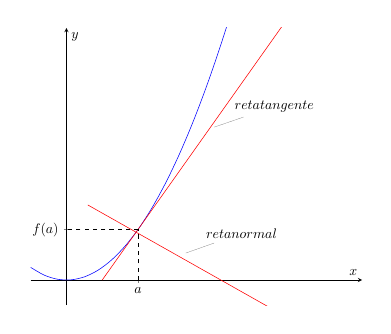
\begin{tikzpicture}[scale=0.5]
\begin{axis}[
 axis lines=middle,
 ticklabel style={fill=white},
%xmin=-1.,%xmax=1.5,
ymin=-0.5, ymax=5,
 xlabel=$x$,ylabel=$y$,
 samples=30,
 smooth,
xtick={1}, ytick={1},
yticklabels={$f(a)$},   xticklabels={$a$},
 width=10cm]
\coordinate  (x2) at (e,1);
\coordinate  (x1) at (0,1);
\addplot[blue, domain=-0.5:5] {x^2};
\addplot[red, domain=0.5:5] {2*x- 1};
\addplot[red, domain=0:5, rotate=-10] {-0.5*x+ 3/2 +0.15};
\node[pin= 30:{$\text{reta tangente}$}] at (axis cs:2,{2*(2)-1}) {};
\node[pin= 30:{$\text{reta normal}$}] at (axis cs:1.6,{-0.5*2+3/2 }) {};
\draw[dashed] (1,0)--(1,1)--(0,1);
\end{axis}
\end{tikzpicture}
\end{Figure}
\end{tcolorbox}

\subsection*{Propriedades Básicas}
\begin{tcolorbox}
\begin{multicols}{3}
$\dfrac{d}{dx}(c)=0$\\[0.5cm]
$\dfrac{d}{dx}\left(x^n\right)= nx^{n-1}$\\[0.5cm]
%$\dfrac{d}{dx}e^x=e^x$\\[0.5cm]
$(c\cdot f)'= cf'$\\[0.5cm]
$(f\pm g)'=f\pm g'$\\[0.5cm]
$(f\cdot g)'=f\cdot g' + g\cdot f'$\\[0.5cm]
$\left(\dfrac{f}{g}\right)'=\dfrac{g\cdot f'-f\cdot g'}{g^2}$
\end{multicols}
\end{tcolorbox}

\subsection*{Derivada de funções Logarítmicas e Exponenciais}
\begin{tcolorbox}
\begin{multicols}{3}
$\dfrac{d}{dx}\left(a^x\right)=a^x\ln{a}$\\[0.5cm]
$\dfrac{d}{dx}\left(e^{x}\right)=e^x$\\[0.5cm]
$\dfrac{d}{dx}\left(\ln{x}\right)=\dfrac{1}{x},\quad x>0$\\[0.5cm]
$\dfrac{d}{dx}\left(\ln{|x|}\right)=\dfrac{1}{x},\quad x>0$\\[0.5cm]
$\dfrac{d}{dx}\left(\log_a{x}\right)=\dfrac{1}{x\ln{a}},\quad x>0$\\[0.5cm]
\end{multicols}
\end{tcolorbox}

\subsection*{Derivada de funções Trigonométricas}
\begin{tcolorbox}
\begin{multicols}{3}
$\dfrac{d}{dx}\left(\sin{x}\right)=\cos{x}$\\[0.5cm]
$\dfrac{d}{dx}\left(\cos{x}\right)=-\sin{x}$\\[0.5cm]
$\dfrac{d}{dx}\left(\tan{x}\right)=\sec^2{x}$\\[0.5cm]
$\dfrac{d}{dx}\left(\csc{x}\right)=-\csc{x}\cot{x}$\\[0.5cm]
$\dfrac{d}{dx}\left(\sec{x}\right)=\sec{x}\tan{x}$\\[0.5cm]
$\dfrac{d}{dx}\left(\cot{x}\right)=-\csc^2{x}$\\
\end{multicols}
\end{tcolorbox}

\subsection*{Derivada de funções Trigonométricas inversas}
\begin{tcolorbox}
\begin{multicols}{3}
$\dfrac{d}{dx}\left(\sin^{-1}{x}\right)=\dfrac{1}{\sqrt{1-x^2}}$\\[0.5cm]
$\dfrac{d}{dx}\left(\cos^{-1}{x}\right)=-\dfrac{1}{\sqrt{1-x^2}}$\\[0.5cm]
$\dfrac{d}{dx}\left(\tan^{-1}{x}\right)=\dfrac{1}{1+ x^2}$\\[0.5cm]
$\dfrac{d}{dx}\left(\csc^{-1}{x}\right)=-\dfrac{1}{x\sqrt{x^2-1}}$\\[0.5cm]
$\dfrac{d}{dx}\left(\sec^{-1}{x}\right)=\dfrac{1}{x\sqrt{x^2-1}}$\\[0.5cm]
$\dfrac{d}{dx}\left(\cot^{-1}{x}\right)=-\dfrac{1}{1+x^2}$\\
\end{multicols}
\end{tcolorbox}

\subsection*{Regra da Cadeia e consequências}
\begin{tcolorbox}
\begin{teorema}[Regra da Cadeia]
Se $F(x)=f(g(x))$ é derivável em $x$ então
\begin{align*}
    F'(x)=\dfrac{d}{dx}\left(f(g(x))\right)=f'(g(x))\cdot g'(x).
\end{align*}
\end{teorema}
\subsubsection*{Consequências}
\begin{multicols}{2}
$\dfrac{d}{dx}\left(\left[f(x)\right]\right)^n=n\left(\left[f(x)\right)\right]^{n-1}f'(x)$\\[0.5cm]
$\dfrac{d}{dx}\left(e^{f(x)}\right)=f'(x)e^{f(x)}$\\[0.5cm]
$\dfrac{d}{dx}\left(\ln\left[f(x)\right]\right)=\dfrac{f'(x)}{f(x)}$\\[0.5cm]
$\dfrac{d}{dx}\left(\sin\left[f(x)\right]\right)=f'(x)\cos\left[f(x)\right]$\\[0.5cm]
$\dfrac{d}{dx}\left(\cos\left[f(x)\right]\right)=-f'(x)\sin\left[f(x)\right]$\\[0.5cm]

$\dfrac{d}{dx}\left(f(x)^{g(x)}\right)= f(x)^{g(x)}\left( \frac{g(x)f'(x)}{f(x)}+\ln\left[f(x)\right]g'(x)\right)$\\
\end{multicols}
\end{tcolorbox}
